\newcolumntype{C}[1]{>{\Centering}p{#1}}
\def\Tab#1#2#3{\small\tabular{C{#1}}\rule[-1.5mm]{0pt}{5mm}\textbf{#2}\\
    \hline\rule[0mm]{0pt}{4mm}#3\rule[-2mm]{0pt}{2mm}\endtabular}
\seticonparams{entity}{
    shadow=false,
    fillcolor=blue!10,
    fillstyle=solid,
    framesep=0pt}

\subsection{Intermodule Dependencies}
\subsubsection{Top Level Structures}
It was apparent from the briefing and requirements that the application would be most suited to a data-centred repository system with the data stored on a distinct central remote server that would be accessed as and when required by the applications running on the separate android phones. The particular aspect of the same data being available to all instances of the android application simultaneously was the main reason the centred data model being chosen. Due to the nature of caches no data can be considered unique to a single user, instead with all users having needs to access the same data. To handle this centralised data a bespoke webserver was created to handle access to a MySQL database to store all data necessary for the android application to run. 

\begin{figure}[h!]
    \centering
    \begin{tabular}{c}
    \entity{database}[\Tab{3cm}{Database}{(SQLite Database)}]
    \hspace{5mm}
    \entity{server}[\Tab{3cm}{Server}{(Webserver)}]
    \hspace{5mm}
    \tabular{C{1mm}}
    \pnode(0,2){arrowtop}
    \pnode(0,-2){arrowbottom}
    \endtabular
    \hspace{5mm}
    \entity{model}[\Tab{3cm}{Model}{(Application's\\functionality)}]
    \hspace{5mm}
    \entity{gui}[\Tab{3cm}{Graphical User Interface}{
        \entity{controller}[\Tab{25mm}{Controller}{(User Input)}] \\[5mm]
        \entity{view}[\Tab{25mm}{View}{(Application Output)}]
    }]
    \end{tabular}
    {\small
        \ncline[arrowscale=1.5]{<->}{database}{server}
        \ncline[arrowscale=1.5,linestyle=dashed]{-}{arrowtop}{arrowbottom}
        \ncline[arrowscale=1.5]{<->}{server}{model}
        \ncline[arrowscale=1.5]{<-}{model}{controller}
        \ncline[arrowscale=1.5]{->}{model}{view}
    }
    \caption{Data flow of the top level of the system, showing the application and server separated by the dashed line, with a clearly visible breakdown of the application into the Model, Controller and View.}
\end{figure}

Due to the requirements of also having a website with much of the functionality that is also required within the application, the decision have a database and separate server was deemed necessary. By having this split structure, both the website and application can have a common interaction point for the data centred model, to help reduce data access concurrency problems as well as having common methods for the same data access regardless of whether the application or website is making access request for data within the database.

\begin{figure}[h!]
    \centering
    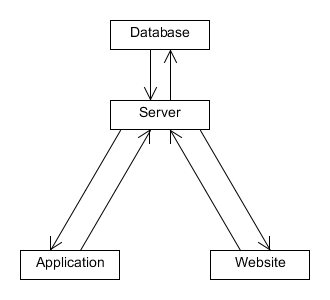
\includegraphics[width=0.6\textwidth]{imdfig2}
    \caption{Top level dataflow for the overall system including a centralised database and server and the application and website which interact with server separately.}
\end{figure}

\newpage
\subsubsection{Model Decomposition}
Due the centralised nature of the data, the Models main function is to make basic get and set requests of the server and parse those results through the use of a json parser ready for the results to be sent to the controller and view of the GUI. This method means that no data is truly stored within the Model of the application, and instead it is only used to control the data flow and interpretation. The Model contains five classes: ServerRequests, CurrentUser, User, Login and Cache. The ServerRequests class contains the majority of the get and set methods required by the application. Each class can then call one of these classes to either retrieve data or send data to the server to be used without needed to interpret the data that the server itself uses.

\begin{figure}[h!]
    \centering
    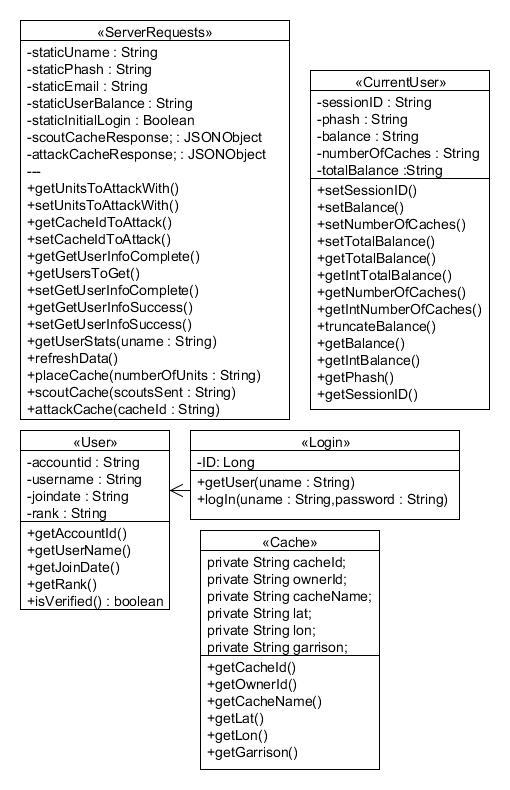
\includegraphics[width=0.7\textwidth]{imdfig3}
    \caption{Showing the properties and methods of classes within the Model component.}
\end{figure}

\subsubsection{Graphical User Interface Decomposition}
The graphical user interface is the largest and most complex component of the application, facilitating user interaction with the application as well as displaying all the possible actions the user can take and results of those actions. The java class Window is the primary class within the GUI with most other GUI related classes inheriting from the Window class.

\begin{figure}[h!]
    \centering
    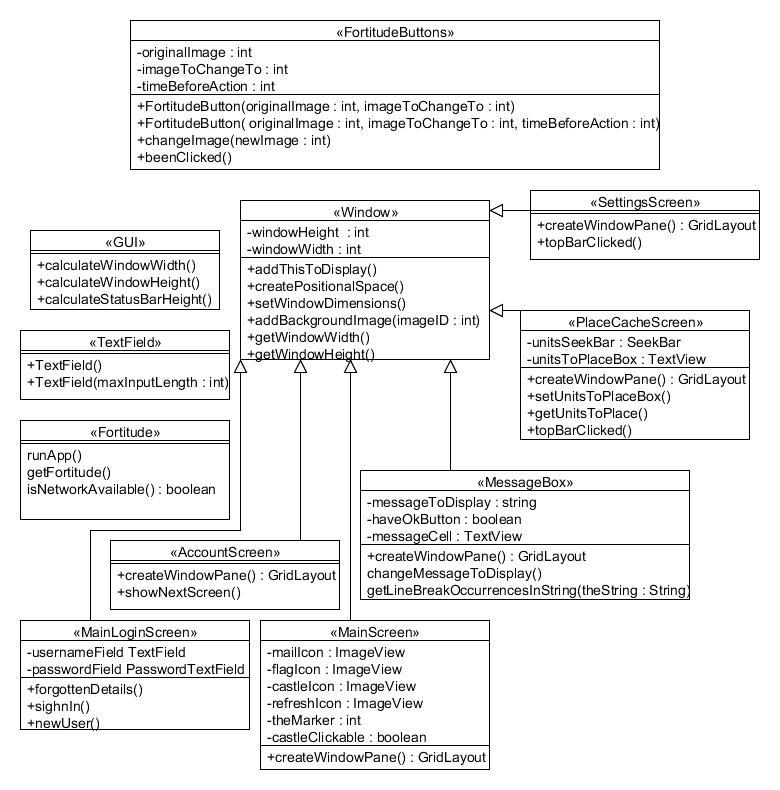
\includegraphics[width=\textwidth]{imdfig4}
    \caption{Properties, classes, methods and Inheritance of the GUI component of the Application.}
\end{figure}


\begin{figure}[h!]
    \centering
    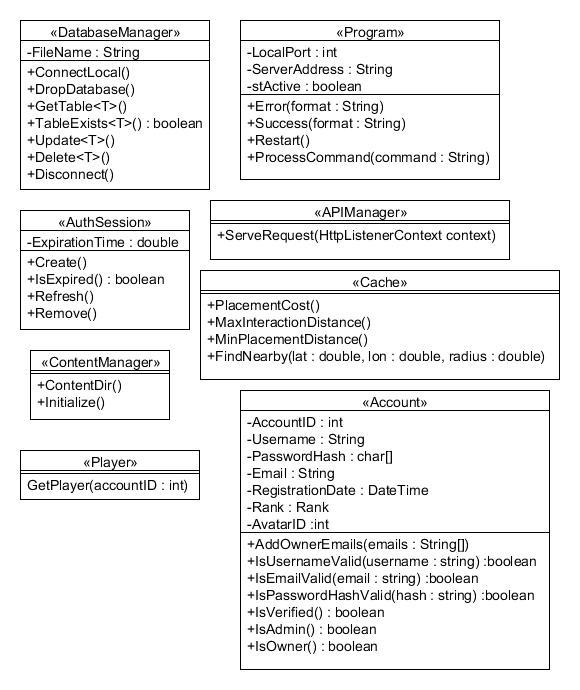
\includegraphics[width=0.8\textwidth]{imdfig5}
\end{figure}
